\documentclass{article}

\usepackage{lipsum} % Package to generate dummy text throughout this template
\usepackage{graphicx, subfig}
\usepackage[sc]{mathpazo} % Use the Palatino font
\usepackage[T1]{fontenc} % Use 8-bit encoding that has 256 glyphs
\linespread{1.05} % Line spacing - Palatino needs more space between lines
\usepackage{microtype} % Slightly tweak font spacing for aesthetics

\usepackage[hmarginratio=1:1,top=26mm,columnsep=20pt]{geometry} % Document margins
\usepackage{multicol} % Used for the two-column layout of the document
\usepackage[labelfont=bf,textfont=it]{caption} % Custom captions under/above floats in tables or figures

\usepackage{geometry}
\usepackage{multicol}
\usepackage{graphicx, subfig}
\usepackage[sc]{mathpazo} % Use the Palatino font
\usepackage[T1]{fontenc} % Use 8-bit encoding that has 256 glyphs
\linespread{1.05} % Line spacing - Palatino needs more space between lines
\usepackage{microtype} % Slightly tweak font spacing for aesthetics

\usepackage[hmarginratio=1:1,top=26mm,columnsep=20pt]{geometry} % Document margins

\usepackage[labelfont=bf,textfont=it]{caption} % Custom captions under/above floats in tables or figures
\usepackage{booktabs} % Horizontal rules in tables
\usepackage{float} % Required for tables and figures in the multi-column environment - they need to be placed in specific locations with the [H] (e.g. \begin{table}[H])
\usepackage{hyperref} % For hyperlinks in the PDF

\usepackage{lettrine} % The lettrine is the first enlarged letter at the beginning of the text
\usepackage{paralist} % Used for the compactitem environment which makes bullet points with less space between them

\usepackage{fancyhdr} % Headers and footers
\pagestyle{fancy} % All pages have headers and footers
\fancyhead{} % Blank out the default header
\fancyfoot{} % Blank out the default footer
\fancyhead[C]{Florida Department of Health $\bullet$ Alachua County } % Custom header text
\fancyfoot[RO,LE]{\thepage} % Custom footer text


\usepackage{Sweave}
\begin{document}
\Sconcordance{concordance:mosquitoRainTempArticle.tex:mosquitoRainTempArticle.Rnw:%
1 39 1 1 0 2 1 1 16 38 1 1 7 1 3 17 1 1 4 9 1 1 6 1 3 19 1 1 8 1 2 10 1 %
1 8 1 2 11 1 1 26 1 2 15 1 1 6 1 3 18 1 1 9 1 2 7 1 1 9 1 2 9 1 1 37 1 %
2 28 1}




\begin{center}
\begin{huge}
Modelling mosquito population in Alachua County\\
\end{huge}
\begin{large}
\vspace{8mm}
Joe Brew, Anthony Dennis, Paul Myers
\vspace{8mm}
\end{large}
\end{center}

\noindent \emph{54\% of the variation in mosquito population in Alachua County can be explained by a  model which takes into account minimum daily temperature and rainfall over a range of prior days.}

\begin{multicols}{2}
\setkeys{Gin}{width=0.49\textwidth}
\section*{Introduction}
Precipitation and temperature variation are known causal predictors for the size of mosquito populations, and the associated human risk of infection with mosquito-borne illness.  Many researchers have constructed complex mathemtical models to predict both the magnitude of an area's mosquito population\footnote{Annelise Tran et al. A Rainfall- and Temperature-Driven Abundance Model for Aedes albopictus Populations. International Journal of Environmental Research and Public Health (Impact Factor: 2). 01/2013; 10(5):1698-719.} as well as the risk for specific arbovirus.
\footnote{Ruiz, MO, et al. Local impact of temperature and precipitation on West Nile virus infection in Culex species mosquitoes in northeast Illinois, USA. Parasites & Vectors 2010, 3:19} 
\footnote{Hosen MB, Morse AP. A weather-driven model of malaria transmission. Malaria Journal 2004, 3:32}
\footnote{Beck-Johnson, LM et al. The Effect of Temperature on Anopheles Mosquito Population Dynamics and the Potential for Malaria Transmission. PLoS ONE 8(11): e79276.}
Though these models are useful for establishing the parameters by which certain mosquito populations grow and infect, their external applicability at the local level is low due to a diversity in species and climate conditions across national, state, and even county lines. \\

\noindent Given that a predictive climate-based modelling for mosquito populations in \textbf{north} Florida\footnote{The Florida Medical Entomology Laboratory carries out extensive mosquito population surveillance using groundwater and other independent predictors in south Florida: http://mosquito.ifas.ufl.edu/Index.htm} has never been carried out (to the authors' knowledge)\footnote{Important disclaimer: "authors' knowledge" is admittedly very limited}, the following represents a first attempt at using precipitation and temperature to estimate the size of the local mosquito population at any given time.  We simulate more than 65,000 linear and 65,000 log-linear models using 148 trap collection dates of 6-10 traps over six summers.  Our best result yields a model which explains 53.8\% of the variation in mosquito population in Alachua County traps.

\section*{Methods}
Data were collected on three key variables for the period of March 1st, 2008 through December 1st, 2013: \\

\textbf{Trapped mosquitoes} were provided by Clarke Scientific, in contract with the Florida Department of Health in Alachua County. These were collected and reported weekly every summer. \\

\textbf{Daily rainfall} was "webscraped" from www.wunderground.com using R\footnote{R Core Team (2013). R: A language and environment for statistical computing. R Foundation for Statistical Computing, Vienna, Austria. URL www.R-project.org/. Full code available upon request: Joseph.Brew@FLHealth.gov} \\

\textbf{Daily minimum temperature} was acquired using the "weatherData" package in R\footnote{Narasimhan, Ran. Package 'weatherData' version 0.3 (2014-01-31)}\\

Both rainfall and temperature readings come from the Gainesville Regional Airport, whereas the 10 mosquito trap sites are scattered throughout Alachua County (see Figure 1).

\begin{figure}[H]
\begin{center}  
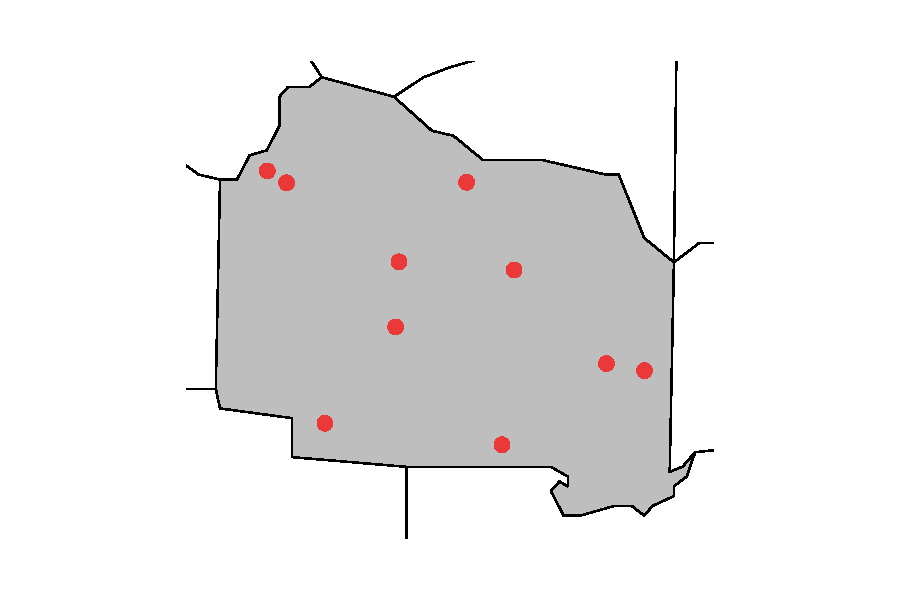
\includegraphics{mosquitoRainTempArticle-003}
\caption{Mosquito trap locations}
\end{center}
\end{figure}

Model construction was approached in two distinct ways:\\

\textbf{Linear}: The first batch of simulations had the model parameters of a simple multivariable linear regression: \\

$\hat{Y}=\alpha+\beta_1 X_1+\beta_2 X_1$ \\

Where $\hat{Y}$= the number of mosquitoes per trap, $\beta_1 X_1$= cumulative rainfall for the period of A through B, $\beta_2 X_1$= the lowest minimum daily temperature for the period of C through D.  \\

A, B, C, D (date ranges) were set as all combinations of 5 through 20 days prior to the date of trap collection.  This produced 256 unique date ranges for both $\beta_1$ as well as $\beta_2$.  All potential combinations  of $\beta_1$ and $\beta_2$ ($256^2$ or 65,536 unique models) were analyzed in a simple linear regression model, and retrospectively ranked for goodness of fit by their unadjusted R-squared values.  \\


\textbf{Log-Linear}: The second batch of simulations was identical, but in this case the natural logarithm of the mean number of mosquitoes per trap was used as $\hat{Y}$ instead of the simple mean number of mosquitoes per trap.  



\section*{Results}
\subsection*{Predictors}


\subsection*{Linear}
65,536 unique models were produced and compared for the linear approach, yielding R-squared values of 0.09 to 0.43 for the linear models (Figure 2).

\begin{figure}[H]
\begin{center}  
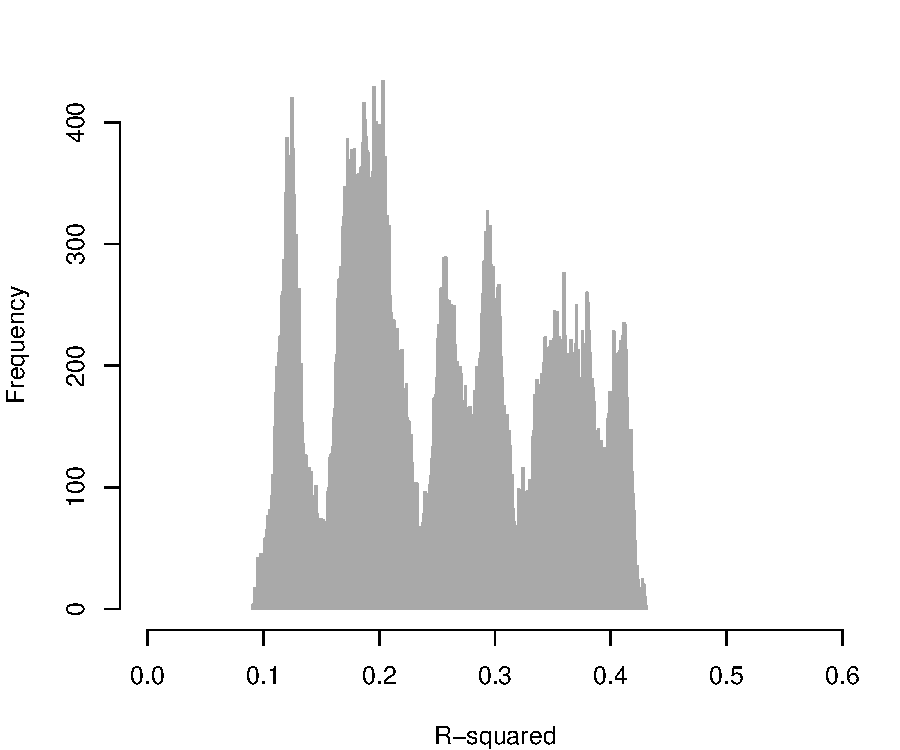
\includegraphics{mosquitoRainTempArticle-005}
\caption{Distribution of linear model R-squared values}
\end{center}
\end{figure}



Of the linear models compared, the one with the best R-squared value (0.43) contained the following estimates:\\

$\beta_1$= cumulative rainfall for the period 16-36 days prior to trap collection 

$\beta_1$= minimum temperature in the period 16-31 days prior to trap collection 

The resulting complete formula was: \\

$\hat{Y}= -234.105 + \beta_1(53.74) + \beta_2(3.496) $ \\


Cumulative rainfall for the simulation-determined best model date ranges exhibited a linear bivariate association with mosquitoes per trap.
\begin{figure}[H]
\begin{center}  
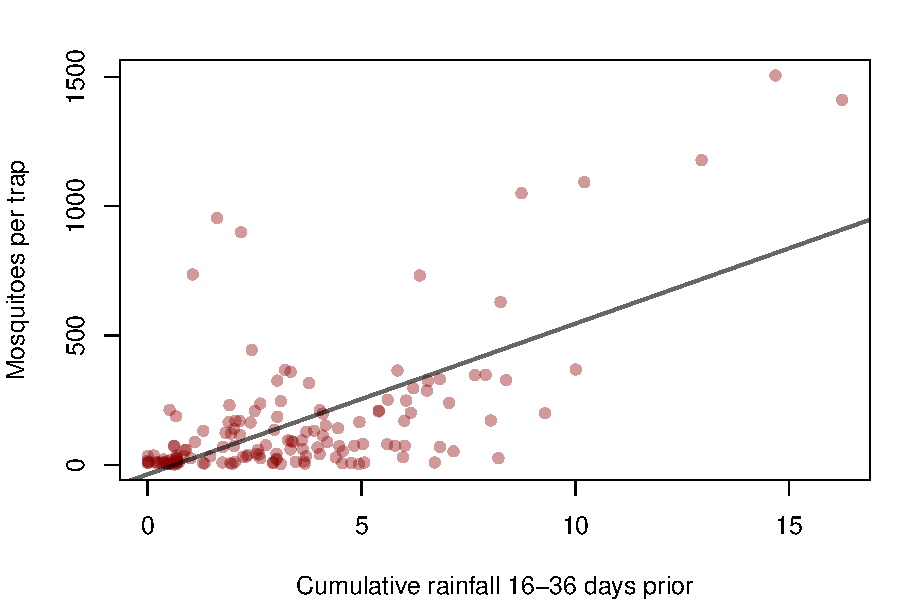
\includegraphics{mosquitoRainTempArticle-006}
\caption{Rainfall and mosquitoes per trap}
\end{center}
\end{figure}

Though minimum temperature for the best model date range exhibited a more exponential shape, transformation yielded only marginally better results. On the other hand, tests yielded a significantly better fit when log-transforming the outcome variable (mosquitoes per trap) instead of the predictor. 

\vfill
\columnbreak

\begin{figure}[H]
\begin{center}  
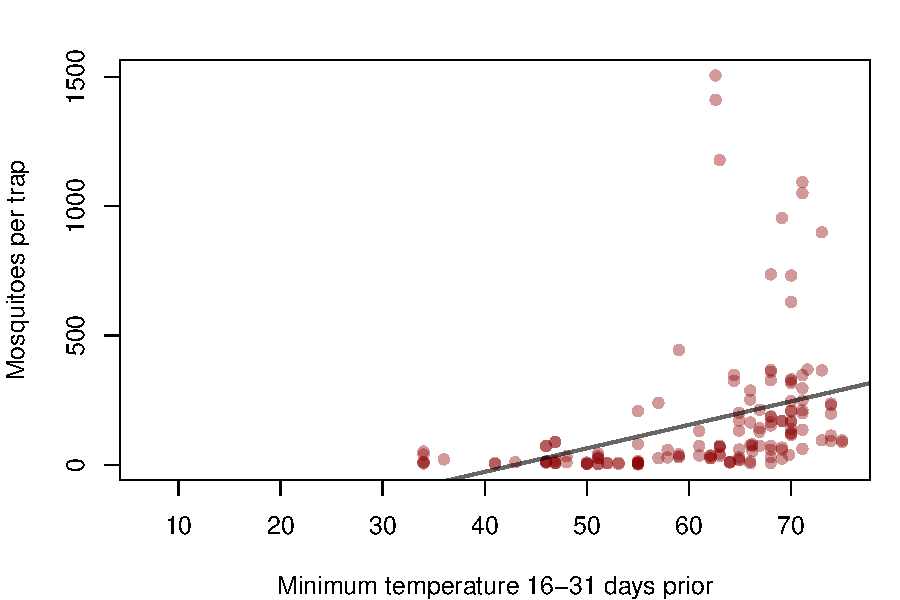
\includegraphics{mosquitoRainTempArticle-007}
\caption{Minimum temperature and mosquitoes per trap}
\end{center}
\end{figure}


The linear approach underestimated peaks and produced many nonsensical negative estimations, particularly in winter months.  Though imperfect, this model does explain 43\% of the variation in mosquito population:

\end{multicols}
\setkeys{Gin}{width=1.0\textwidth}

\begin{figure}[H]
\begin{center}  
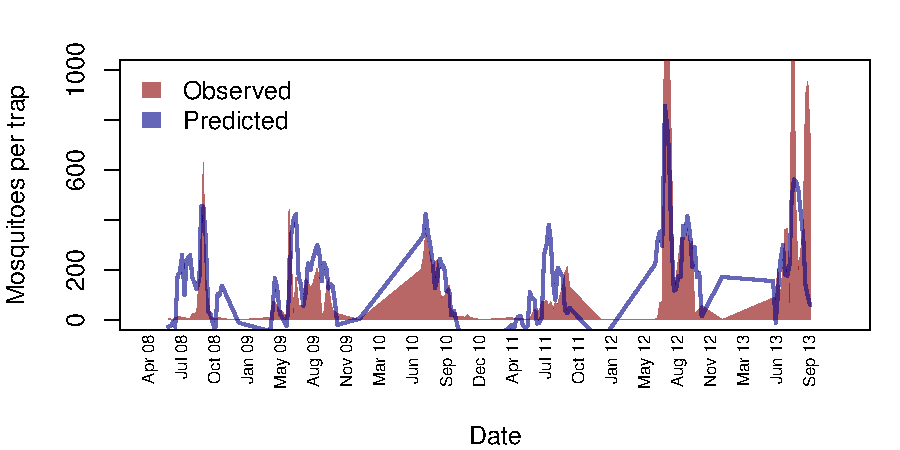
\includegraphics{mosquitoRainTempArticle-008}

\caption{Time series: predicted versus observed (best linear model)}
\end{center}
\end{figure}


\newpage

\begin{multicols}{2}
\setkeys{Gin}{width=0.48\textwidth}

\subsection*{Log-Linear}
65,536 unique models were also produced and compared for the log-linear approach, yielding R-squared values of 0.30 to 0.54 (Figure 3).
\vspace{-3mm}
\begin{figure}[H]
\begin{center}  
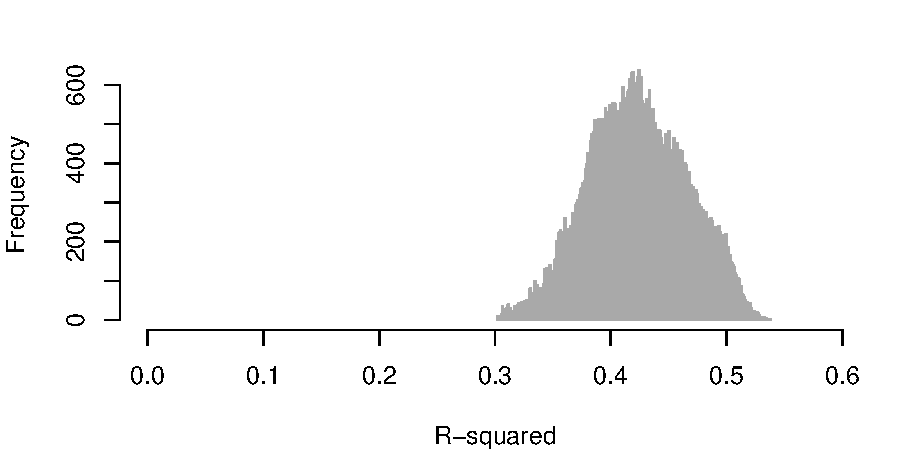
\includegraphics{mosquitoRainTempArticle-009}
\caption{Distribution of log-linear model R-squared values}
\end{center}
\end{figure}

The best log-linear model (R-squared = 0.54) contained the following estimates:\\

$\beta_1$= cumulative rainfall for the period 17-37 days prior to trap collection 

$\beta_1$= minimum temperature in the period 14-32 days prior to trap collection 

The resulting complete formula was: \\

$\hat{Y}= exp(-1.121+ \beta_1(0.200) + \beta_2(0.074)) $ \\


Cumulative rainfall for the simulation-determined best model date ranges exhibited a linear bivariate association with the natural logarithm of mosquitoes per trap, though it was heteroskadistic and could perhaps benefit from a log-log transformation.
\vspace{-3mm}
\begin{figure}[H]
\begin{center}  
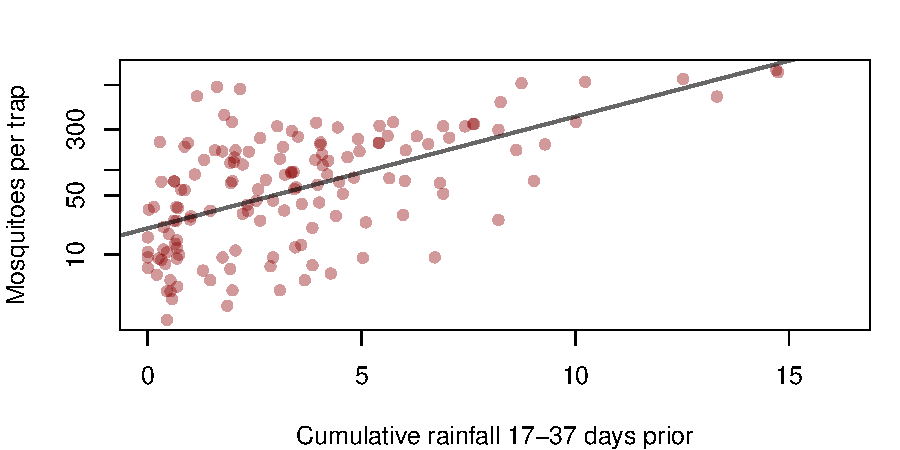
\includegraphics{mosquitoRainTempArticle-010}
\caption{Rainfall and mosquitoes per trap}
\end{center}
\end{figure}

\vspace{-10mm}

\begin{figure}[H]
\begin{center}  
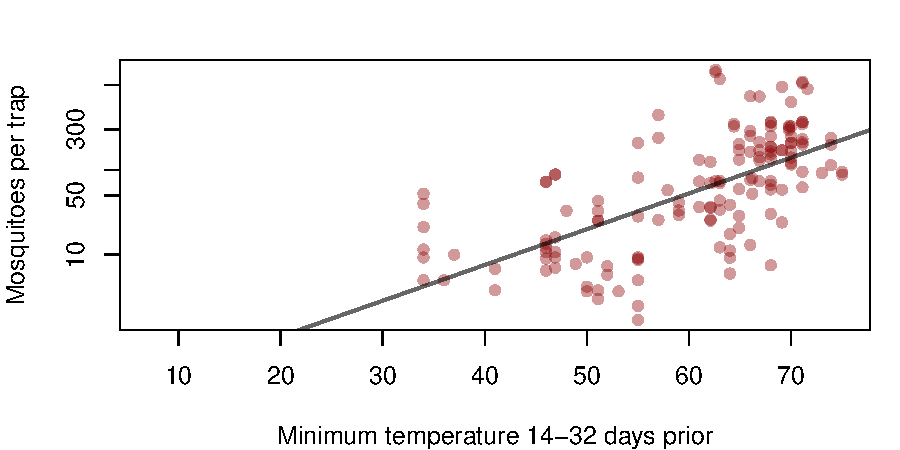
\includegraphics{mosquitoRainTempArticle-011}
\caption{Minimum temperature and mosquitoes per trap}
\end{center}
\end{figure}

\end{multicols}
\setkeys{Gin}{width=1.0\textwidth}

\vspace{-3mm}
\begin{figure}[H]
\begin{center}  
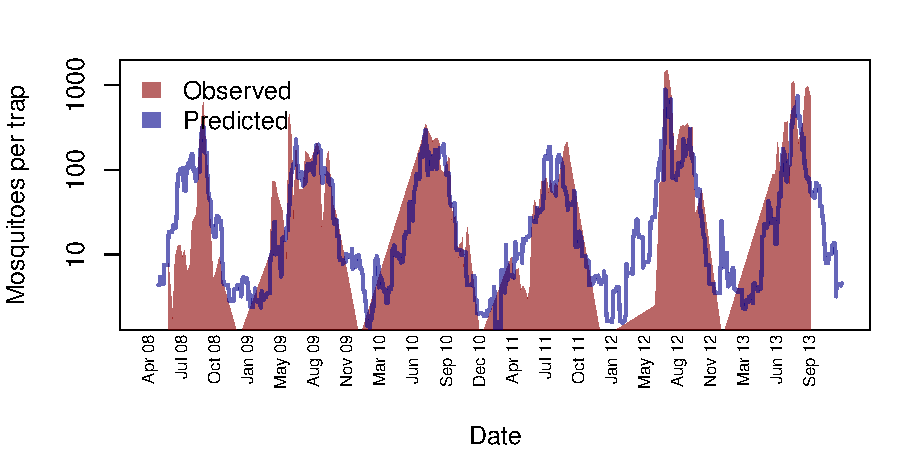
\includegraphics{mosquitoRainTempArticle-012}

\caption{Time series: predicted versus observed (best log-linear model)}
\end{center}
\end{figure}

\newpage

\begin{multicols}{2}
\setkeys{Gin}{width=0.48\textwidth}


\section*{Discussion}
Though not nearly as robust as more complex models, which take into account specific species' lifecycles and mating habits as a function of weather (and at times yield R-squared values as high as 0.8)\footnote{Gong Honfei et al. A Climate Based Moquito Population Model. Proceedings of the World Congress on Engineering and Computer Science 2007
WCECS 2007, October 24-26, 2007, San Francisco, USA}, simple linear modelling performed fairly well in terms of predicting general trends.  It correctly predicted the large peaks in mosquito population in both 2012 and 2013 (with some slight underestimation), as well as the smaller peaks in other years.  \\

A log-linear model represented a significant improvement, though further variable-specific transformation might yield even better results. \\

Of particular note, this model is valuable in that its independent variable range minimum values are 14 days prior to trap collection.  In other words, mosquito population spikes can be predicted at least 14 days in advance, granting public health authorities time both to inform the population and take precautionary methods (spraying, etc.).\\

\subsection*{Further research}
To fully understand the dynamics of mosquito populations in North Florida, further study is needed.  The population numbers of vectors of specific emerging arboviruses (such as Dengue, Chikungunya and West Nile Fever) should be individually modelled so as to better understand the threat therein.  Collaboration with entomologist and arbovirus specialists could lead to the inclusion and refinement of further potentially predictive variables.  Finally, trap data should be shared among counties so as to ensure more precise modelling througher larger sample size.

\section*{Conclusion}
Given the arrival of new mosquito-borne illnesses in Florida, and the rapid changes in the epidemiology of arbovirus in the south, local governments should pay close attention to the threat posed by summer spikes in mosquito populations.  Public health authorities in  Florida can benefit from predictive modelling to assess and control the threat of spikes in mosquito population weeks in advance.  

\end{multicols}
 

\end{document}
